

%No more than a few pages
%Include:
%- General features of the LHC and the injector chain
%- Luminosity and integrated luminosity
%- could discuss the details of the accelerator and machine parameters


%define these abbreviations here:
%LHC - Large Hadron Collider
The Large Hadron Collider (LHC) \cite{lhc} is
a 27 km circumference collider ring
located at CERN approximately 100 m underground on the 
of French-Swiss border near Geneva, Switzerland.
Its primary goal is to collide protons at very high energies (
the TeV scale)  similar to energies just a few trillionths of a second (?)
after the big bang.  %
The products of these collisions can 
be observed
by several independent but complementary detectors placed at different
points around the ring in order to probe the mechanism
for EWSB as well as to test and probe for new physics beyond the SM.
Since the dynamics of the collisions are governed by quantum mechanical
processes, the types of collision processes of interest cannot be
produced on demand, but instead occur at random with some
probability.
The probability for these processes is typically very small; thus, they are quite
rare (quote a number).
These processes are also short lived, meaning they do not live long
enough to reach the detector and are instead observed indirectly through their
decays. Since multiple physics processes can have the same decay 
signature, it is not possbile to say with certainty that a given 
collision comes from a specific physics process. Instead, 
we must count the number of observed collisions for a given signature
and compare this to the number expected from the 
quantum mechanical probabilities.  If the observed number differs
from the expected, then it could simply suggest that the theoretical expectation
is not well understood or it could suggest the presence of some new physics
process.
In order to make an adequate statement, we must be able to count
enough collisions of the desired signature (say 10 to 1000 depending on the
signature and its backgrounds) 
such that the statistical uncertainty is low.  This places a demand
on the LHC to produce as many collisions as possible, even of these rare
processes. To accomplish this, the LHC is thus designed to collide
protons at a maximum frequency of 40 MHz, or 40 million times per second!
More details about the LHC and collider physics in general are presented
below.



\section{Collider Physics}
\label{sec:lhc_collider_physics}

From the persepective
of a particle physicsist studying the products of particle collisions, we 
are interested in collisions produced at the highest possible energies,
measured by the collision center-of-mass energy, and at the highest possible rates, 
measured by the luminosity.
The center-of-mass energy, $E_{\textrm{CM}}$, is the collision energy 
in the rest frame
of the collision. For head-on collisions with both beams at the same
energy, $E$, like at the LHC, this is simply the sum of the energies, 
or $E_{CM} = 2 E$. So, $E_{\textrm{CM}}$ grows linearly as a function
of the beam energy. This is in contrast with fixed target experiements
where $E_{\textrm{CM}} \propto \sqrt{E}$ and thus grows much more slowly. 
Frequently this is related to the Mandelstam variable,
$s$, which is the squared magnitude of the Lorentz four-vectors
of the incoming collision particles $p_1$ and $p_2$ such that
$s = (p_1+p_2)^2 = E_\textrm{CM}^2$.
The high beam energies required prefer a circular collider (as opposed
to a linear collider) so that the particles may be repeatedly 
accelerated at each cycle using the same hardware.
In order to accelerate the particles, they must be both stable (if you
want them to hang around long enough to collide) and charged (so
that they may respond to electromagnetic steering and acceleration).
This leaves just protons and electrons (and their anti-particles)\footnote{It is also
possible to collide heavy ions, such as lead. In fact, the LHC does collide
heavy ions when it is not colliding protons, though that is not the focus of this
thesis.}.
Electrons and positrons are fundamental particles and thus provide
very clean collisions, but their small mass means that they suffer
from high energy losses due to syncrhotron radiation in response to acceleration. 
Too much synchrotron radiation and the beam could lose too much energy
to be practical. 
This decides the overall radius and size of the collider ring, since a smaller
ring means tighter turns and thus more acceleration\footnote{In fact, 
the LHC uses the same tunnel (which was the same size) as 
the Large Electron-Positron (LEP) Collider and which
operated from 1989 to 2000 but only up to energies of 209 GeV for the reasons
described.}.
Protons and anti-protons are much less affected by synchrotron radiation
and thus can be accelerated to higher energies at a circular collider.
To bend the particles around the ring at high beam energies 
requires tremendously strong dipole magnets. 
Thus, the limiting factor for the energy is ultimately the requirements
on the dipole magnets, which must be superconducting and at the cutting-edge 
of current technology.
To get the particles to these very high energies, the particles
are ultimately accelerated using electromagnetic waves in radio-frequnency cavities.
The beam is chopped up into ``bunches'' separated at regular intervals
to synchronize with the amplitude and ``surf'' the wave.  The frequency
of the radio-frequnecy waves thus determines the bunch spacing.


The luminosity, $L$,  can be thought of as the overall intensity of the beam.
For a colliding beam it may be simply defined as
\begin{equation}
L=f \frac{N_b^2}{4\pi\sigma^2} R
\end{equation}
where $f$ is the collision frequency (related to the bunch spacing and thus
in the MHz radio-frequency range), 
$N_b$ is the number of particles in a bunch (usually 10-100 billion), 
$R$ is a  geometrical factor
taking into account details like the crossing angle of the collision (on the
order of unity),
and $\sigma$ is the transverse size of the bunches\footnote{Not to be confused
with the cross-section in particle physics.} (which 
is usually on the order of tens of microns).
Thus, modern colliders typically have luminosities on the order of 
$10^{30}$ to $10^{34}~\lumiunits$.
The transverse size of the beam is governed by the relativistic 
energy of the beam and is carefully tuned in the LHC
using arrays of focusing magnets. 
The luminosity of the beam is not constant, but instead steadily decreases
as a function of time, $t$:
\begin{equation}
L(t) = L_0 \tau_L\Big( 1- e^{-t/\tau_L} \Big)
\label{eq:lhc_lumi}
\end{equation}
where $L_0$ is the initial luminosity and $\tau_L$ is the lifetime of the 
beam. The finite lifetime (on the order of hours) comes from gradual 
degradation of the beam quality, mainly due to the beam collisions themselves.
As the beam reaches the end of its life, the beam is dumped and a new
run is started. This process is repeated as many times as possible. The 
luminosity is then integrated over time as a measure of how many collisions
were performed (and also how much data was collected).  This can
then be related to the cross-section for a given process, $\sigma$, to estimate
how many events from that process, $N$, would have been produced on average:
\begin{equation}
N=\sigma \int L~ \textrm{d}t
\end{equation}


While it is true that the we desire to increase the luminosity as much
as possible, there is one important subtlety. 
Limitations on the size of the luminosity do not just
come from the collider but also come from the detectors in the form of pileup.
Pileup is the phenomena of multiple collisions occuring during a single
bunch crossing. Since we are trying to make statements about the 
physics of collisions and not bunch crossings, we must be able to 
identify the individual collisions themselves. The typical length of 
a bunch is usually on the order of tens of centimeters while the number of pileup 
collisions per bunch crossing is on the order of ten or more. Furthermore, 
the collisions do not occur inside the detetor, with the decay products
being measured a few centimeters away (?). Thus, to distinguish individual
collisions the detector must be able to extrapolate the tracks of the decay
products back to the collision point with a resolution much less than 
a centimeter. This process is called vertexing and places strict 
requirements on the precision of the tracking systems for any detector
built at a modern collider. An example of the vertexing for a typical
bunch crossing in ATLAS is shown in \fig\ref{fig:lhc_pileup}.
Another issue of pileup is that each collision produces thousands of 
tracks which all contribute to the occupancy of the detector. If the occupancy
is saturated, the detector may not be able to resolve individual tracks
and would thus be useless. This is a serious concern for detectors
at future colliders where problems of pileup will continue to grow.


\section{The LHC Accelerator Complex}

\begin{figure}[ht!]
\centering
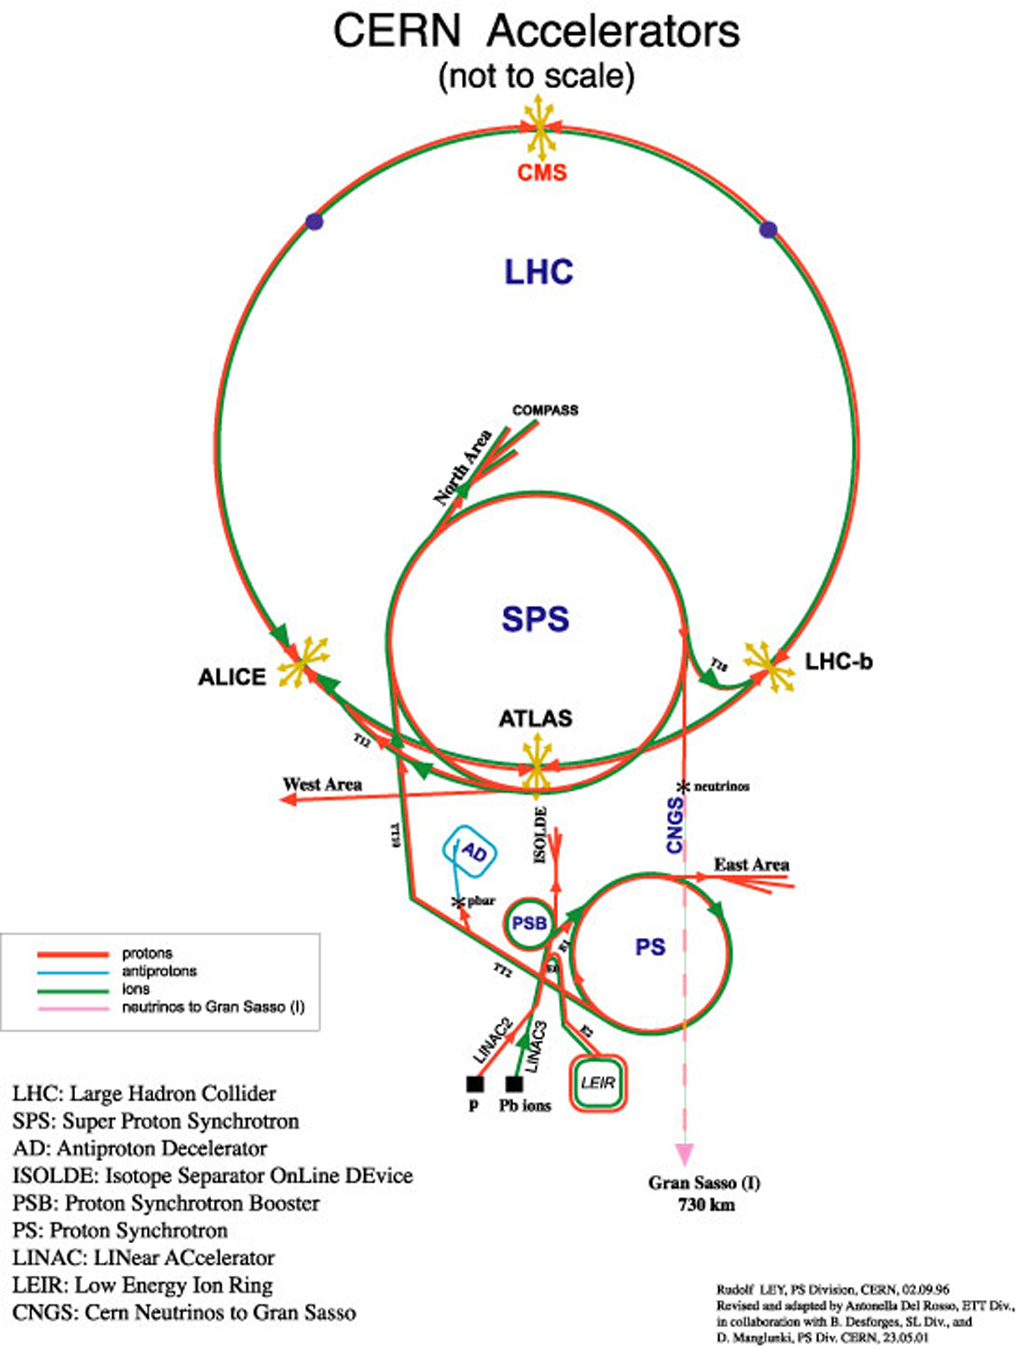
\includegraphics[width=.8\textwidth]{figures/lhc/complex.jpg}
\caption{Diagram of the different accelerators in the CERN accelerator
complex~\cite{lhccomplex}. Those relevant for the LHC are the Linac2, PSB, PS, SPS, and the LHC itself. The ATLAS detector is labeled at the bottom of the LHC ring.}
\label{eq:lhc_complex}
\end{figure}

The LHC was designed to provide proton-proton collisions
at an energy of 14 TeV (7 TeV per beam) 
and a peak luminosity of $10^{34}~\lumiunits$ with a 25 ns collision
bunch spacing (400 MHz).
Protons are collected from hydrogen gas by first stripping away 
the electron in an electric field. The protons are injected
into a series of lower energy accelerators before ultimately 
reaching the LHC to be accelerated to the full energy and 
begin collisions. The various stages of the LHC accelerator
complex are shown in \fig\ref{fig:lhc_complex}.
The protons are accelerated to initially using the LINAC2 linear
accelerator. Next, the protons pass through the circular
Proton Synchrotron Booster (PSB), Proton Synchrotron (PS),
and Super Proton Synchrotron (SPS). Finally, they 
are split into two beams and injected into the LHC
travelling in opposite directions. Once in the LHC
ring they are accelerated to their full energy and then made
to collide at four points along the ring where detectors
are positioned to examine the products of the collisions.
The two general purpose detectors, ATLAS \cite{ATLAS} and CMS \cite{CMS}, 
are positioned at opposite sides of the ring. 
Meanwhile, the two specialized detectors, ALICE \cite{ALICE} 
and LHC-b \cite{LHCB}, are situated at equal points along the ring
nearest ATLAS.
The total injection process takes about 4 minutes.



mention why don't use anti-protons at the LHC.

footnote. Motivation for proton-proton over p-pbar or ee burn rate would be too high. (see slides C)


\section{Data Collection}
%The LHC ran at a center-of-mass energy\footnote{Reduced from the design energy of 14 TeV.} from 2010 to 2011. 
In 2012, the LHC operated at a center-of-mass energy of 8 TeV\footnote{Reduced
from the initial design energy of 14 TeV due to a quenching incident
in the superconducting dipole magnets in 2008 when running at full energy.}
with a bunch spacing of 50 ns with 1.6 to 1.7 $\times 10^{11}$ protons
per bunch, a beam radius of $18.8 \mu$m, and an average peak 
luminosity of $7.7 \times 10^{33}~\lumiunits$ \cite{Lamont:1709796}.
The luminosity lifetime, $\tau_L$, corresponding to \eqn\eqref{eq:lhc_lumi},
ranged from 7 hours to 14 hours during a single run (i.e. the shape
of the exponential changes) \cite{Hostettler:2013qya}.
The peak luminosity recorded per day and the total integrated luminosity 
in 2012 are shown 
on the left and right, respectively, of \fig\ref{fig:lhc_lumi}.
The overall delivered integrated luminosity from the LHC
in 2012 was 23.3 \ifb, while that recorded was 21.7 \ifb. The 
amount of data recorded that is relevant for this thesis
and described in \sec\ref{sec:www} is slightly less at 20.3 \ifb.

The pileup conditions during 2012 were such that an average
of 20.7 collisions occured per bunch crossing. The distribution
of the average interactions per crossing in 2012 are shown in 
\fig\ref{fig:lhc_pileup_recorded}.
show also 7 TeV? mention 7 and 13 TeV runs?


